% Created:  Mon 01 Sep 2014 01:03 PM
% Author:   Josh Wainwright
% Filename: testing.tex

\section{Testing}
\label{sec:testing}

Since the absolute definition of the clusters that the plugin looks for are
somewhat subjective, testing the algorithm for correctness is difficult. The
individual functions and smaller components of the algorithms are tested using
the unit testing framework JUnit \cite{tahchiev2010junit}, and the overall
effectiveness of the clustering algorithms is validated with generated data
files and acceptance testing.

\subsection{Generated Test Files}
\label{sub:generated_test_files}

To try to test the algorithm and get some more quantitative results, it was
performed on a number of simulated test files. These data sets, shown in
Figure~\ref{fig:cam-tests} were produced by \citet{karypis1999chameleon} for
testing their Chameleon clustering algorithm. The algorithm was found to
identify 4 clusters in image (a) and a single cluster image (b), but performed
poorly in the final two.

\begin{figure}[tbh]
	\centering
	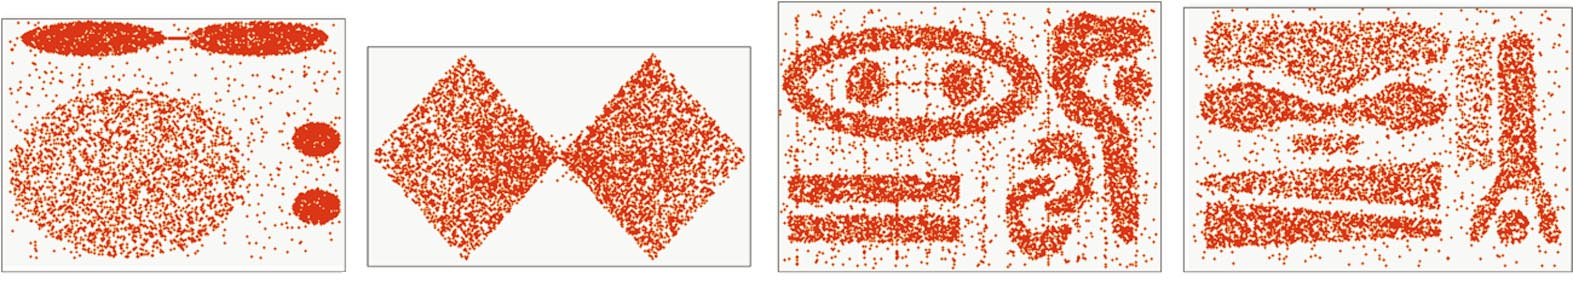
\includegraphics[width=0.9\linewidth]{cam-tests.png}
	\caption[Manually generated data sets for testing]{Manually generated data
		sets for testing. The images (a), (b), (c) and (d) above are used to
		test the algorithm for this project and for a number of other studies
		in clustering.}\label{fig:cam-tests}
\end{figure}

These particular datasets have been used to test a number of clustering
algorithms and so they provide a helpful benchmark with which these algorithms
can be compared. It is unfortunate that this algorithm fails to cope with the
complex structures that are present in the second two images, but shows that it
is more specifically tailored than the more general algorithms that use these
as tests. The clusters that the algorithm failed to identify lie too close
together meaning that the propagation step is able to cross from one cluster to
another.

The same effect is seen in images (a) and (b) where there is a link between
what would, otherwise, be separate clusters. This means the algorithm reports
these as a single object.

Another testing data set was created, similar to the final two images above,
but with more spacing to see how the algorithm would cope. An image of this set
is shown in Figure~\ref{fig:testing-image2a}.

% \begin{figure}[tbh]
% 	\centering
% 	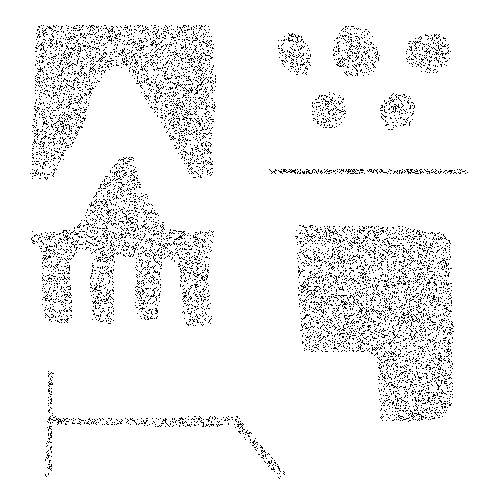
\includegraphics[width=0.5\linewidth]{testing-image2a.png}
% 	\caption[Custom generated data set for testing clustering
% 		algorithm.]{Custom generated data set for testing clustering
% 		algorithm. This data set is similar to that shown above, but
% 		has more space between clusters. The number of points in this
% 		data set is appropriately \num{14000}.} \label{fig:testing-image2a}
% \end{figure}

\begin{figure}[tbhp]
	\centering
	\begin{subfigure}[b]{0.3\textwidth}
		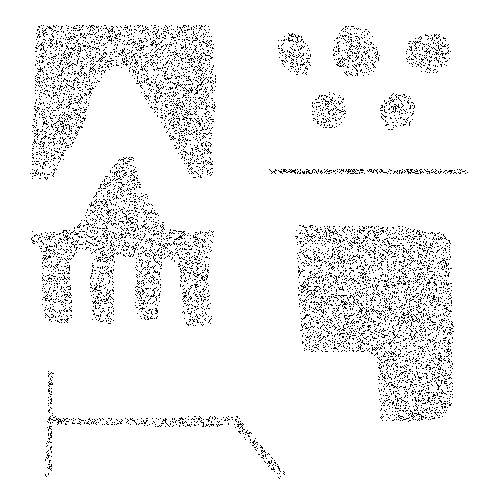
\includegraphics[width=\textwidth]{testing-image2a.png}
		\caption{}\label{fig:testing-image2a}
	\end{subfigure}%
	\quad
	\begin{subfigure}[b]{0.3\textwidth}
		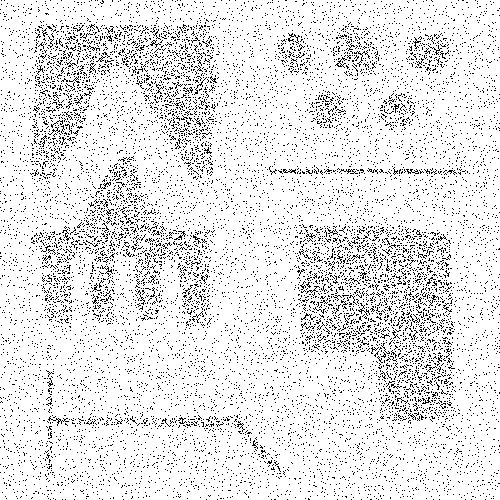
\includegraphics[width=\textwidth]{testing-image2b.png}
		\caption{}\label{fig:testing-image2b}
	\end{subfigure}
	\caption[Custom generated data set for testing clustering
		algorithm.]{Custom generated data set for testing clustering
		algorithm. This data set is similar to that shown above, but
		has more space between clusters. The number of points originally in
		this data set is appropriately \num{14000},
		\subref{fig:testing-image2a}, and random noise is added up to a ratio
		of $1.4:\!1$,~\subref{fig:testing-image2b}.}\label{fig:testing-image2a}
\end{figure}

The results were better with this data set since the propagation step of the
algorithm was halted by the clear space between the clusters. When there is no
noise at all in the data, all of the clusters are located. The amount of noise
can be increased by simply adding random data points which are distributed
evenly across the image space. This is done progressively, adding appropriately
\num{2000} points at a time. The clustering algorithm stops finding the
clusters properly when roughly \num{10000} random points have been added,
Figure~\ref{fig:testing-image2b}. This represents when the signal to noise
ratio is noise $1.4:\!1$.

\subsection{Volunteer Validation}
\label{sub:volunteer_validation}

The first stage of acceptance testing took the form of a sample set of data
that was plotted onto an image using the discrete grid method. This data was
then presented to a number of volunteers who were asked to count the number of
clusters they could identify and then highlight the clusters that they were
able to observe in order of precedence, most defined through to least defined.

Once the volunteer had identified the clusters, the algorithm was performed on
the same set of data and the results compared to the predicted results.
Finally, when the algorithm identified clusters that the volunteers had not,
they were asked to identify which of these they did not consider to be valid
clusters and which were valid clusters that they had missed. The number of
false positive clusters identified by the quadtree algorithm was found, by this
method, to be low.

When using the settings described in Section~\ref{sub:option_sliders}, 100\% of
the clusters identified by the volunteers were able to be located by the
algorithm. Of the clusters that the algorithm found but the volunteers did not,
around 60\% were considered to be valid by the volunteers. These results
suggest that the algorithm is performing well at being able to identify
clusters, but requires some intervention to get the best results (see
Section~\ref{sec:possible_improvements}) and that, in general, the algorithm
does not produce that many false positive results.

\subsection{Researcher Validation}
\label{sub:researcher_validation}

The final stage of acceptance testing was performed to confirm the type of
clusters identified conformed with the actual objects that are being imaged.
This was performed by a researcher working in the medical imaging field who
produced the sample data used in this project.

The feedback from the researcher was very positive with relation to the
performance of the clustering algorithm. In particular the speed of the plugin
to produce results was commented as being much better than existing utilities
that have been written in the MatLab suit \cite{matlab2010}. This means that a
user can make changes to the settings a number of times to get the results
desired without spending long periods of time waiting for the process to
complete.

The clusters that were identified, when given some sample data from current
research, were also confirmed to be in line with the biological theory,
something that only someone with good knowledge in the area could confirm. With
some explanation of the effects of the different settings, the researcher was
able to produce desirable results quickly.

There were a number of suggestions for improvements that were identified. Many
of these would not require large changes to the code base. These are summarised
below.

\begin{description}[style=unboxed]

	\item[Provide a better mapping between the clusters highlighted in the
		image and the results table which summarises the clusters.] \hfill

		The image is colored with each cluster that is found having a different
		colour which then corresponds to a line in the results table. This
		mapping is not clear since the results table does not allow any
		contents other than strings of text. A better solution would be to
		label each of the clusters in the image with a numerical value which
		can then be identified in the table by the cluster id.

		This would require a single extra step during the drawing phase to add
		a text label with the number of the cluster.

	\item[Allow choosing the scale of the image to correspond to the real size
		of the object which is imaged.] \hfill

		A setting in the main UI that allows the user to input a scale would
		mean that the results that are presented in the table would have more
		immediate value. This value would be the dimensions of the image which
		would be able to act as a multiplication factor for the other results.

	\item[Use different clustering algorithms from the same plugin.] \hfill

		As discussed in more detail in Section~\ref{sec:possible_improvements},
		the ability to choose from a number of different algorithms to perform
		the clustering would make the plugin more general purpose, in the event
		that one of them did not cope well with the particular data being
		examined. Adding other algorithms would, currently, require some
		refactoring of the code to separate some of the functionality from the
		algorithm. This would be required so that adding other algorithms was
		simple.

\end{description}
